\section{Monopolar vs Dipolar Stimulation: Quantitative Comparison}
\label{appendix:mono-vs-dipolar}

This appendix provides quantitative evidence supporting the choice of dipolar over monopolar
stimulation, as discussed in Section~\ref{subsec:phantom_head_transfer_model}.

Two stimulation protocols were evaluated through FEM simulations. For both protocols,
a forward transfer matrix $F$ was computed, where each column represents the scalp
voltages measured at the 21 probes (according to the ten-twenty electrode system of the International 
 Federation~\cite{klem-1999}) for one unit source activation (monopole or dipole).
The matrix maps internal electrode activations to surface measurements, forming the
basis for comparing spatial discriminability.

\paragraph*{Monopolar protocol.}
Each electrode $e_i$ ($i = 1, \ldots, 9$) was individually set to $+1$~V while the remaining
8 electrodes were held at $0$~V. This produced 9 simulation cases, yielding a forward
transfer matrix $F_{\text{mono}} \in \mathbb{R}^{21 \times 9}$, where each column
represents the probe response to activating a single electrode.

\paragraph*{Dipolar protocol.}
All $\binom{9}{2} = 36$ distinct electrode pairs were configured as dipoles:
for pair $(e_i, e_j)$ with $i < j$, electrode $e_i$ was set to $+1$~V,
electrode $e_j$ to $-1$~V, and the remaining 7 electrodes to $0$~V.
This produced 36 simulation cases, yielding the forward transfer matrix
$F \in \mathbb{R}^{21 \times 36}$, where each column represents the probe response
to one unit dipole activation.

\subsection{Matrix Properties and Probe Discrimination}

Table~\ref{tab:mono-vs-dip-matrix} compares the fundamental properties of both forward matrices.

\begin{table}[h]
\centering
\caption{Comparison of monopolar and dipolar forward matrix properties.}
\label{tab:mono-vs-dip-matrix}
\begin{tabular}{lcc}
\toprule
\textbf{Property} & \textbf{Monopolar} & \textbf{Dipolar} \\
\midrule
Matrix size & $21 \times 9$ & $21 \times 36$ \\
Rank & 9 & 21 \\
Condition number ($\kappa$) & 128 & 10424 \\
Max singular value & 0.937 & 0.649 \\
Min singular value & $7.3 \times 10^{-3}$ & $6.2 \times 10^{-5}$ \\
\bottomrule
\end{tabular}
\end{table}

The monopolar matrix has full column rank (9) but only spans a 9-dimensional
subspace of $\mathbb{R}^{21}$. Its lower condition number ($\kappa = 128$) is
misleading: the fundamental limitation is insufficient rank to represent arbitrary
21-dimensional probe patterns. The dipolar matrix achieves full row rank (21),
spanning the entire probe measurement space. Its poor condition number ($\kappa \approx 10424$)
reflects redundancy among the 36 dipole orientations --- precisely the information-rich
basis from which selection algorithms will extract well-conditioned subsets.

The critical difference lies in \emph{probe discrimination}. For each probe, we computed
the coefficient of variation (CV = $\sigma / \lvert\mu\rvert$) across all stimulation
cases. A high CV indicates that probe responses vary significantly with source location,
enabling spatial discrimination. A low CV indicates nearly uniform responses regardless
of which source is active.

\begin{table}[h]
\centering
\caption{Probe discrimination statistics across all 21 measurement locations.\nota{chequear los valores, los tenia anotados en un papel, pero no tenía el desarollo de las cuentas ahí}}
\label{tab:mono-vs-dip-cv}
\begin{tabular}{lcc}
\toprule
\textbf{Metric} & \textbf{Monopolar} & \textbf{Dipolar} \\
\midrule
Mean CV across probes & 44\% & 645\% \\
Min CV (worst discrimination) & 26\% & 91\% \\
Max CV (best discrimination) & 67\% & 2607\% \\
Mean probe std (mV) & 29.3 & 34.4 \\
\bottomrule
\end{tabular}
\end{table}


\subsection{Field Visualization}

Figures~\ref{fig:mono-cases}--\ref{fig:dip-correlation} show the electric potential
distribution and correlation analysis for all stimulation cases. Visual inspection
reveals that monopolar fields exhibit highly similar patterns regardless of source
location, while dipolar fields show diverse orientations and polarity distributions.

\begin{figure}[p]
\centering
\includegraphics[width=1\textwidth]{../../02_Images/monopolar_grid.pdf}
\caption{Electric potential distributions for the 9 monopolar stimulation cases.
Fields exhibit similar patterns regardless of which electrode is activated.}
\label{fig:mono-cases}
\end{figure}

\begin{figure}[h]
\centering
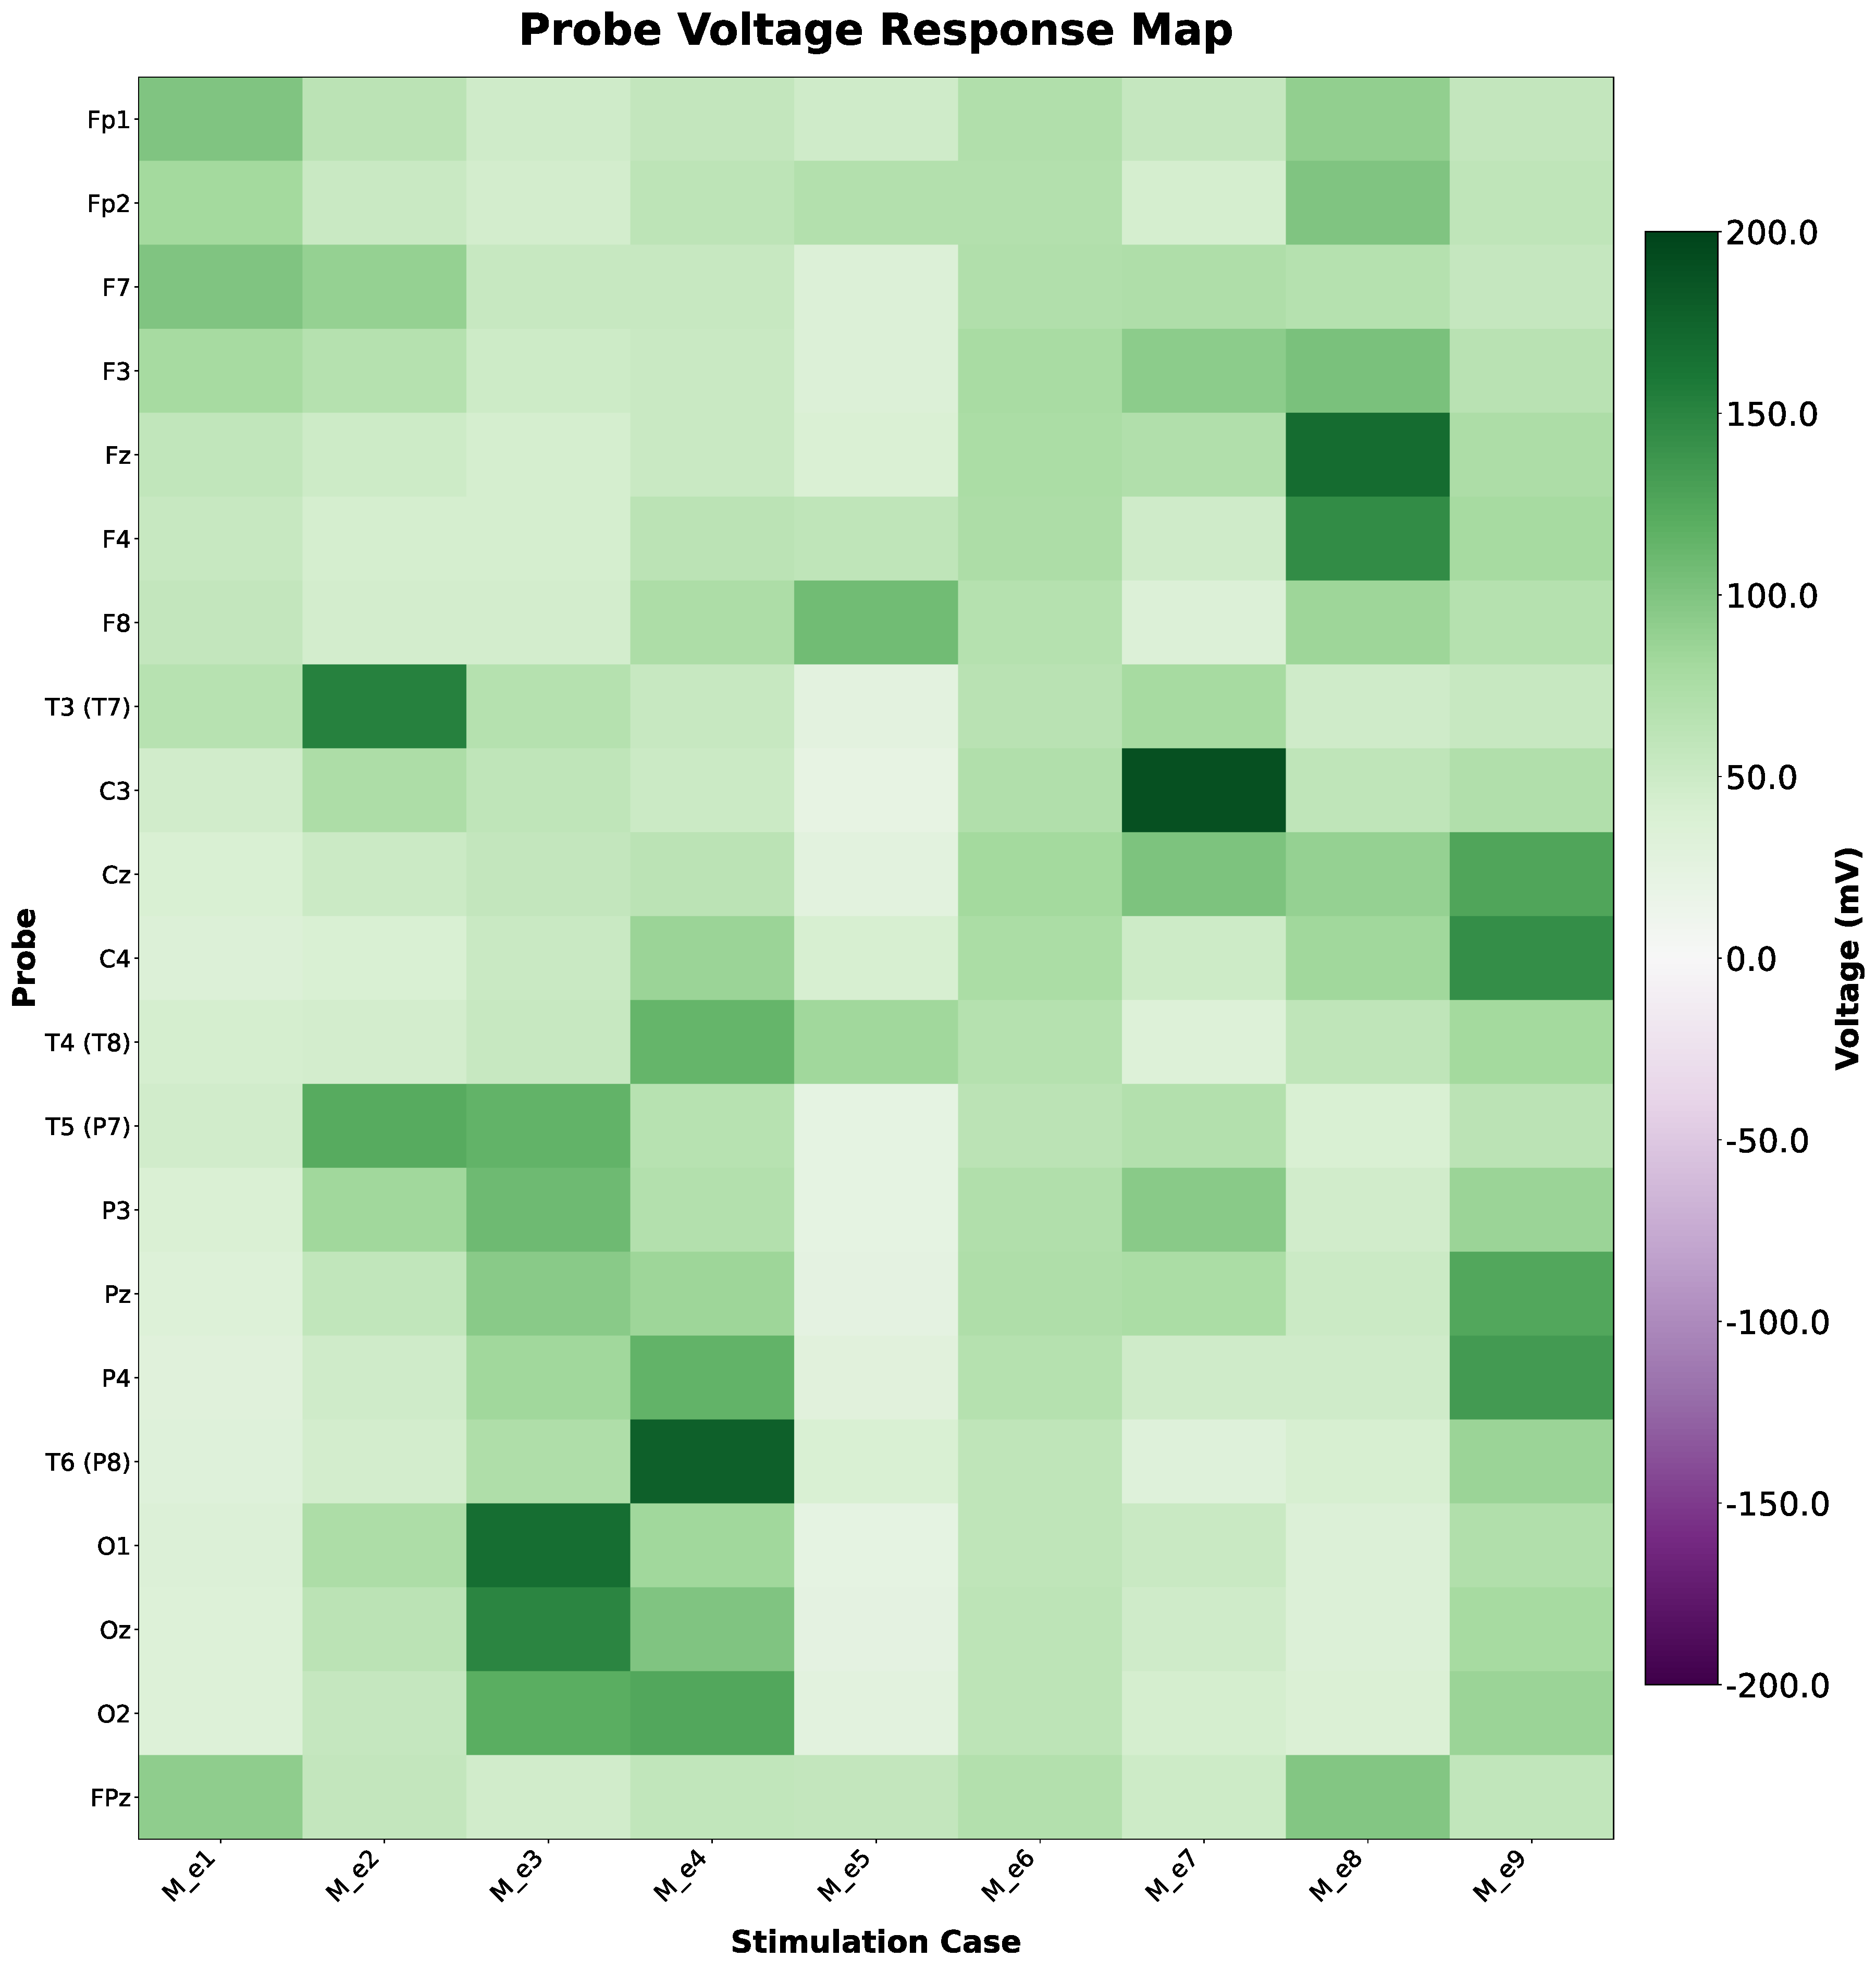
\includegraphics[width=1\textwidth]{../../02_Images/mono_F_matrix_heatmap.pdf}
\caption{Heatmap of probe voltage responses for monopolar stimulation. Each row
represents one of the 21 probes, each column represents one of the 9 electrode
activations, with color indicating measured voltage magnitude.}
\label{fig:mono-heatmap}
\end{figure}

\begin{figure}[p]
\centering
\includegraphics[width=1\textwidth]{../../02_Images/dipolar_grid.pdf}
\caption{Electric potential distributions for the 36 dipolar stimulation cases.
Fields show diverse orientations and polarity distributions.}
\label{fig:dip-cases}
\end{figure}

\begin{figure}[h]
\centering
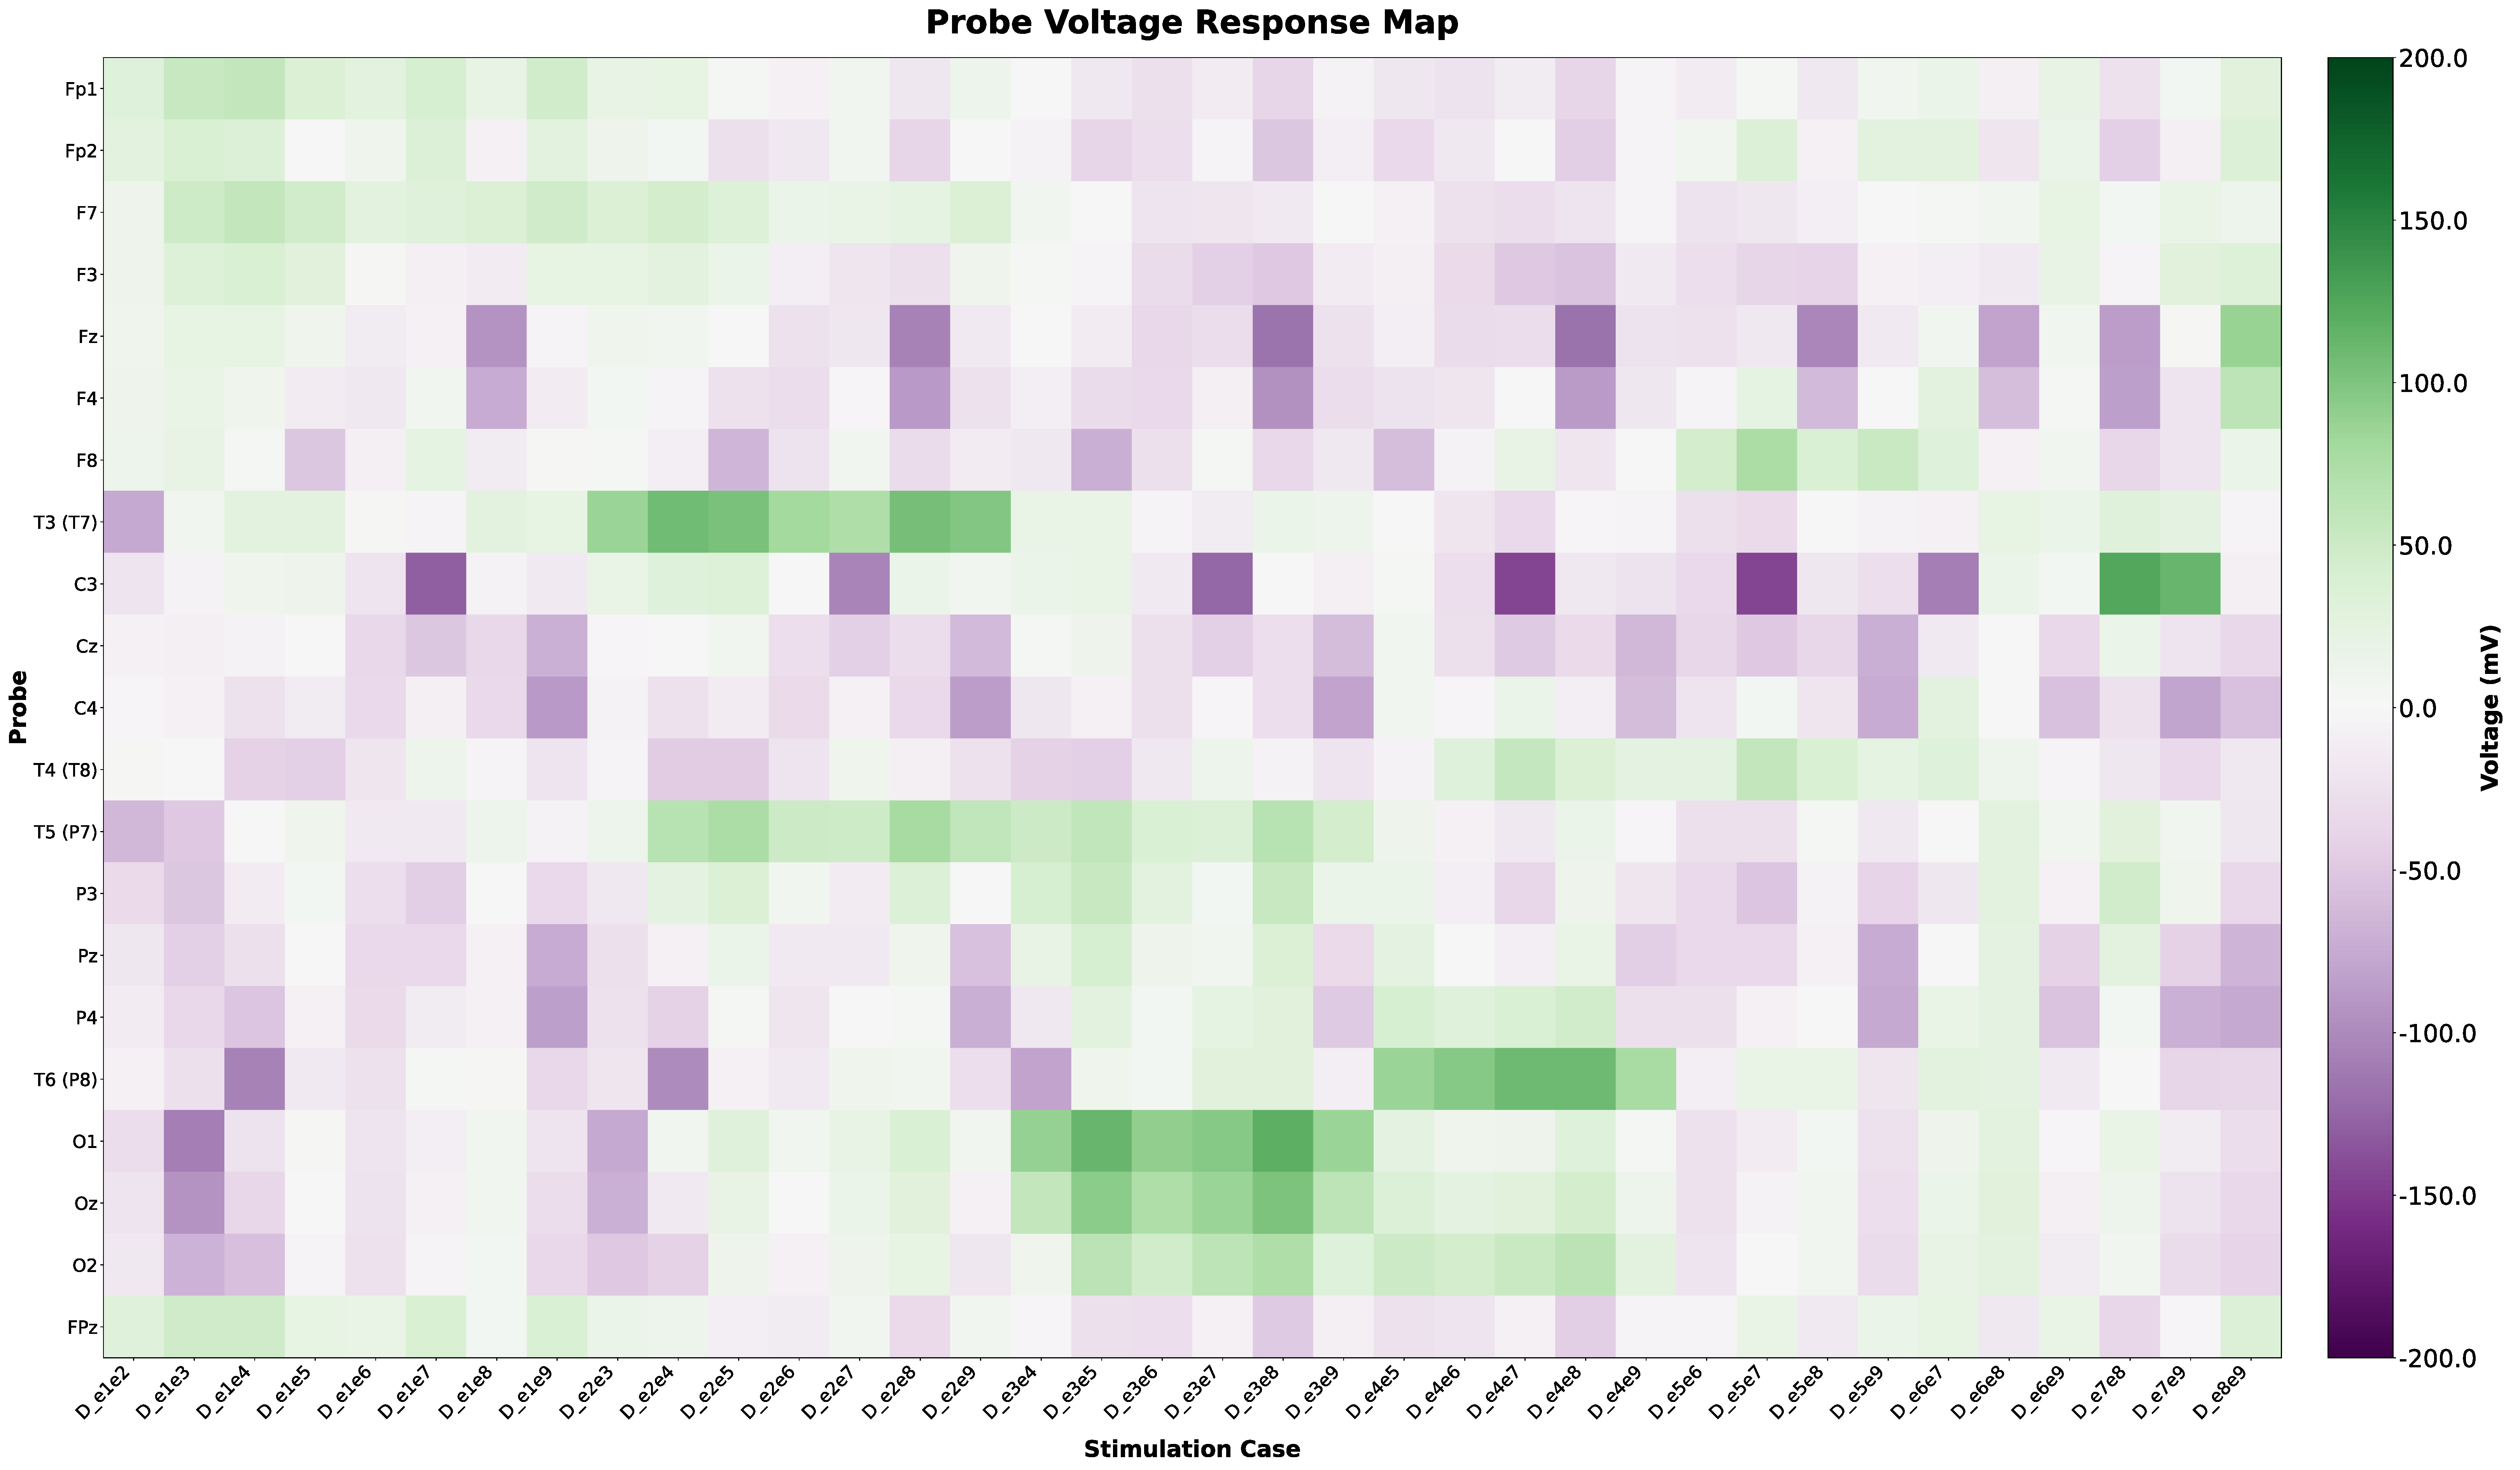
\includegraphics[angle=270,width=0.9\textwidth]{../../02_Images/dip_F_matrix_heatmap.pdf}
\caption{Heatmap of probe voltage responses for dipolar stimulation. Each row
represents one of the 21 probes, each column represents one of the 36 dipole
configurations, with color indicating measured voltage magnitude.}
\label{fig:dip-heatmap}
\end{figure}

This visual observation is quantified by the correlation matrices in
Figures~\ref{fig:mono-correlation} and~\ref{fig:dip-correlation}.
The monopolar matrix shows high correlation among columns (\nota{mean $r = 0.94$}), confirming
that the 9 activation patterns are nearly indistinguishable. The dipolar matrix shows
much lower correlation (\nota{mean $r = 0.31$}), indicating far more distinct probe patterns.

\begin{figure}[h]
\centering
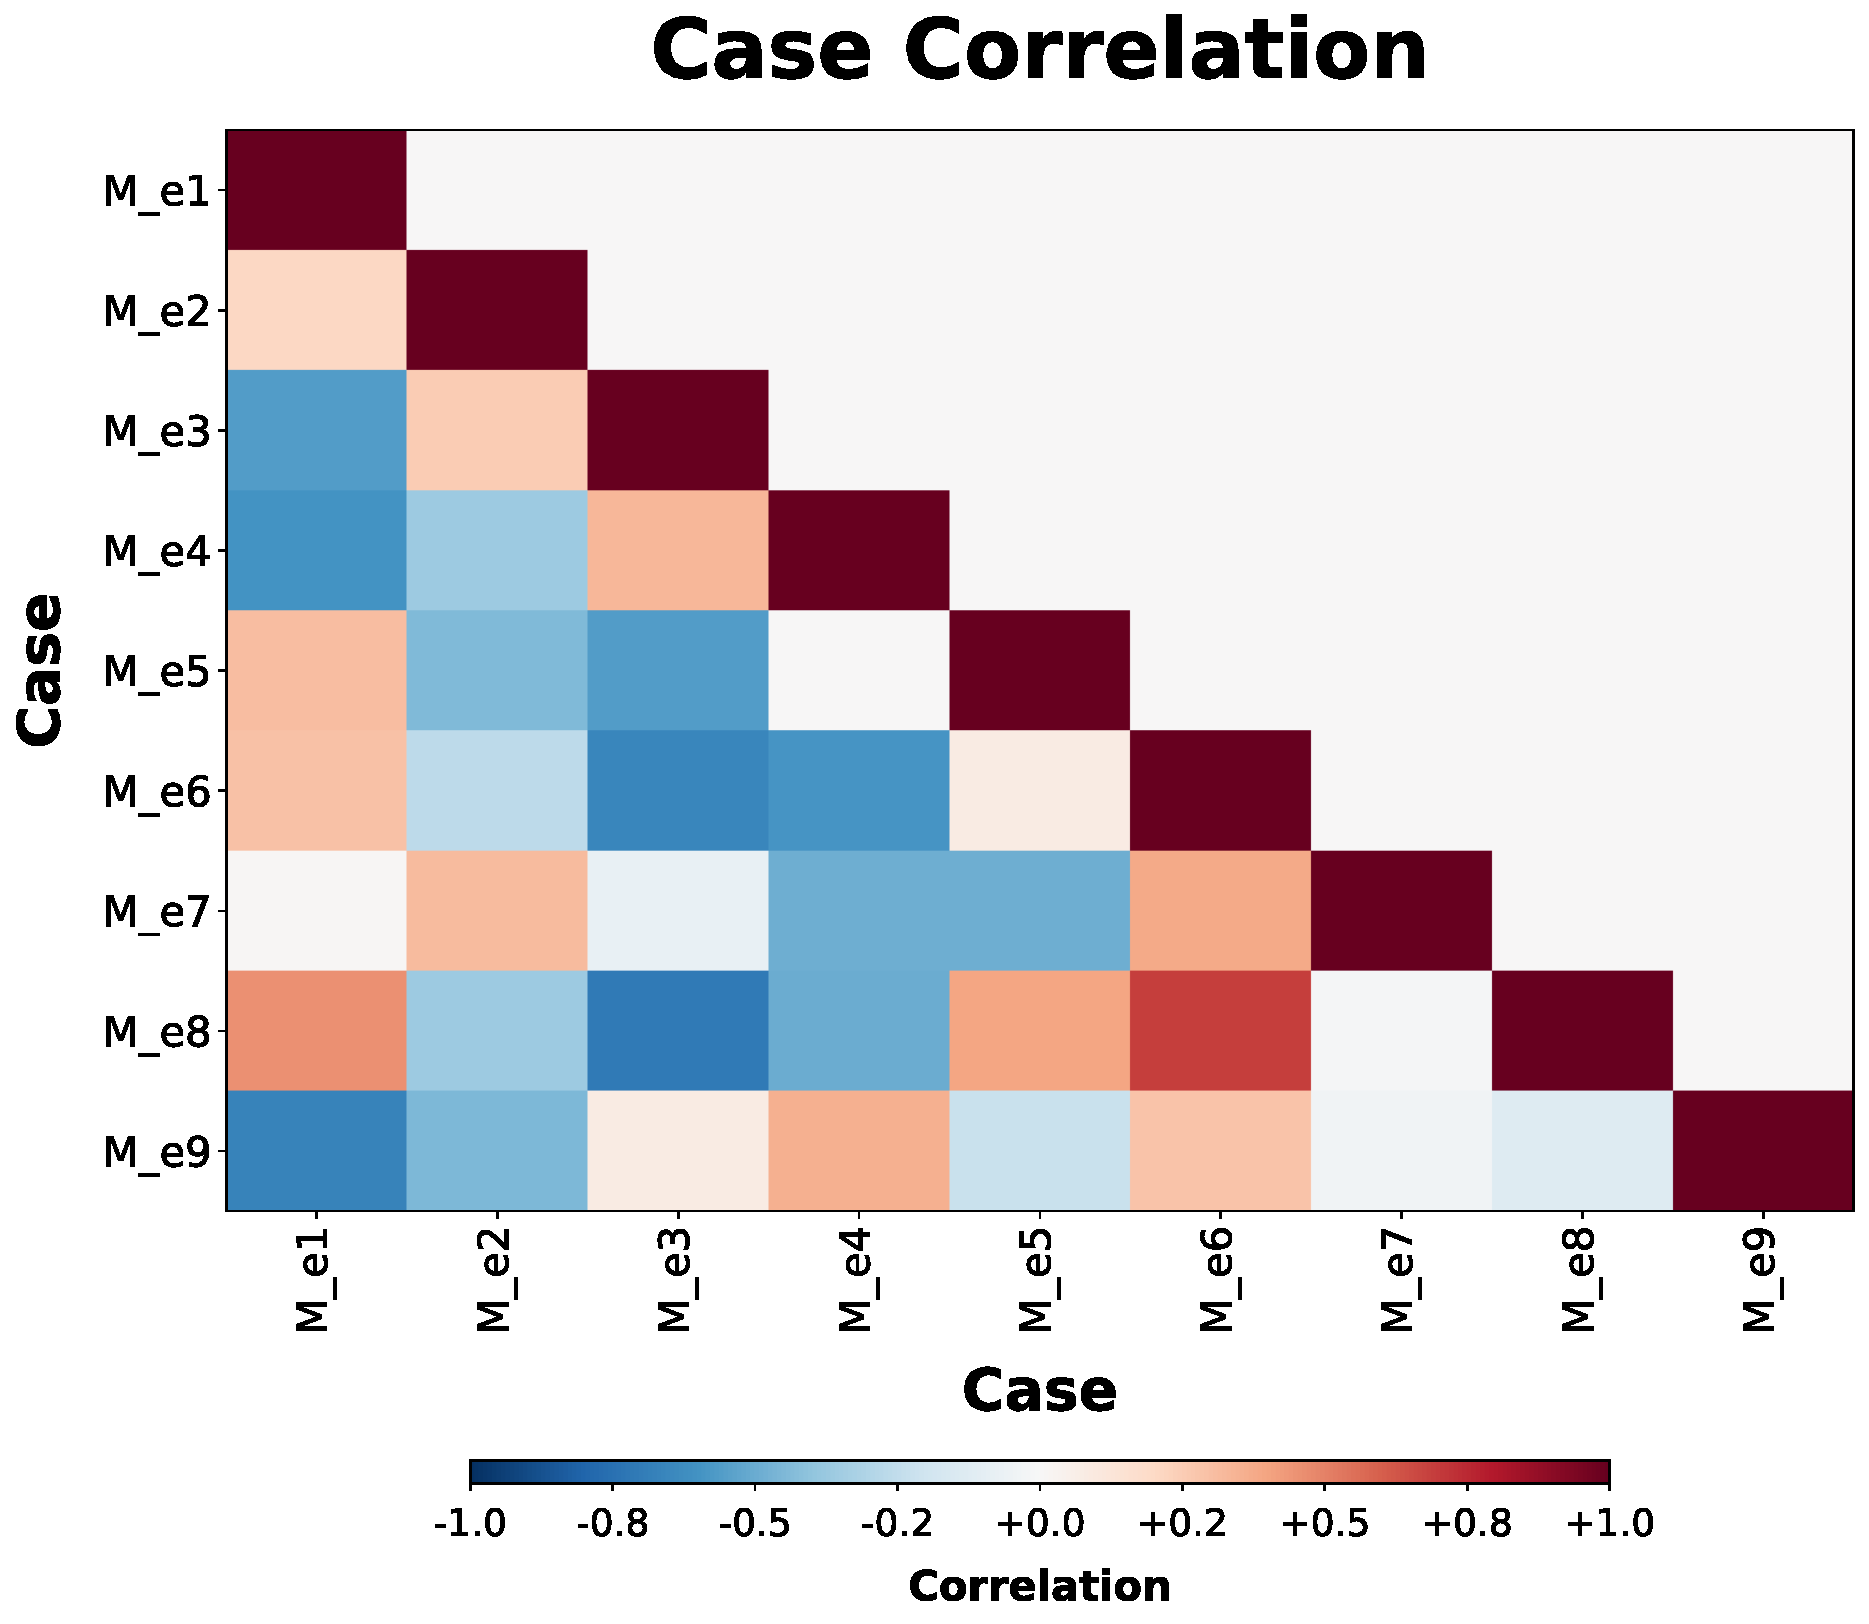
\includegraphics[width=\textwidth]{../../02_Images/mono_correlation_heatmap.pdf}
\caption{Correlation matrix for monopolar stimulation patterns.
Columns are highly correlated ($r \approx 0.94$), indicating similar probe responses.}
\label{fig:mono-correlation}
\end{figure}

\begin{figure}[h]
\centering
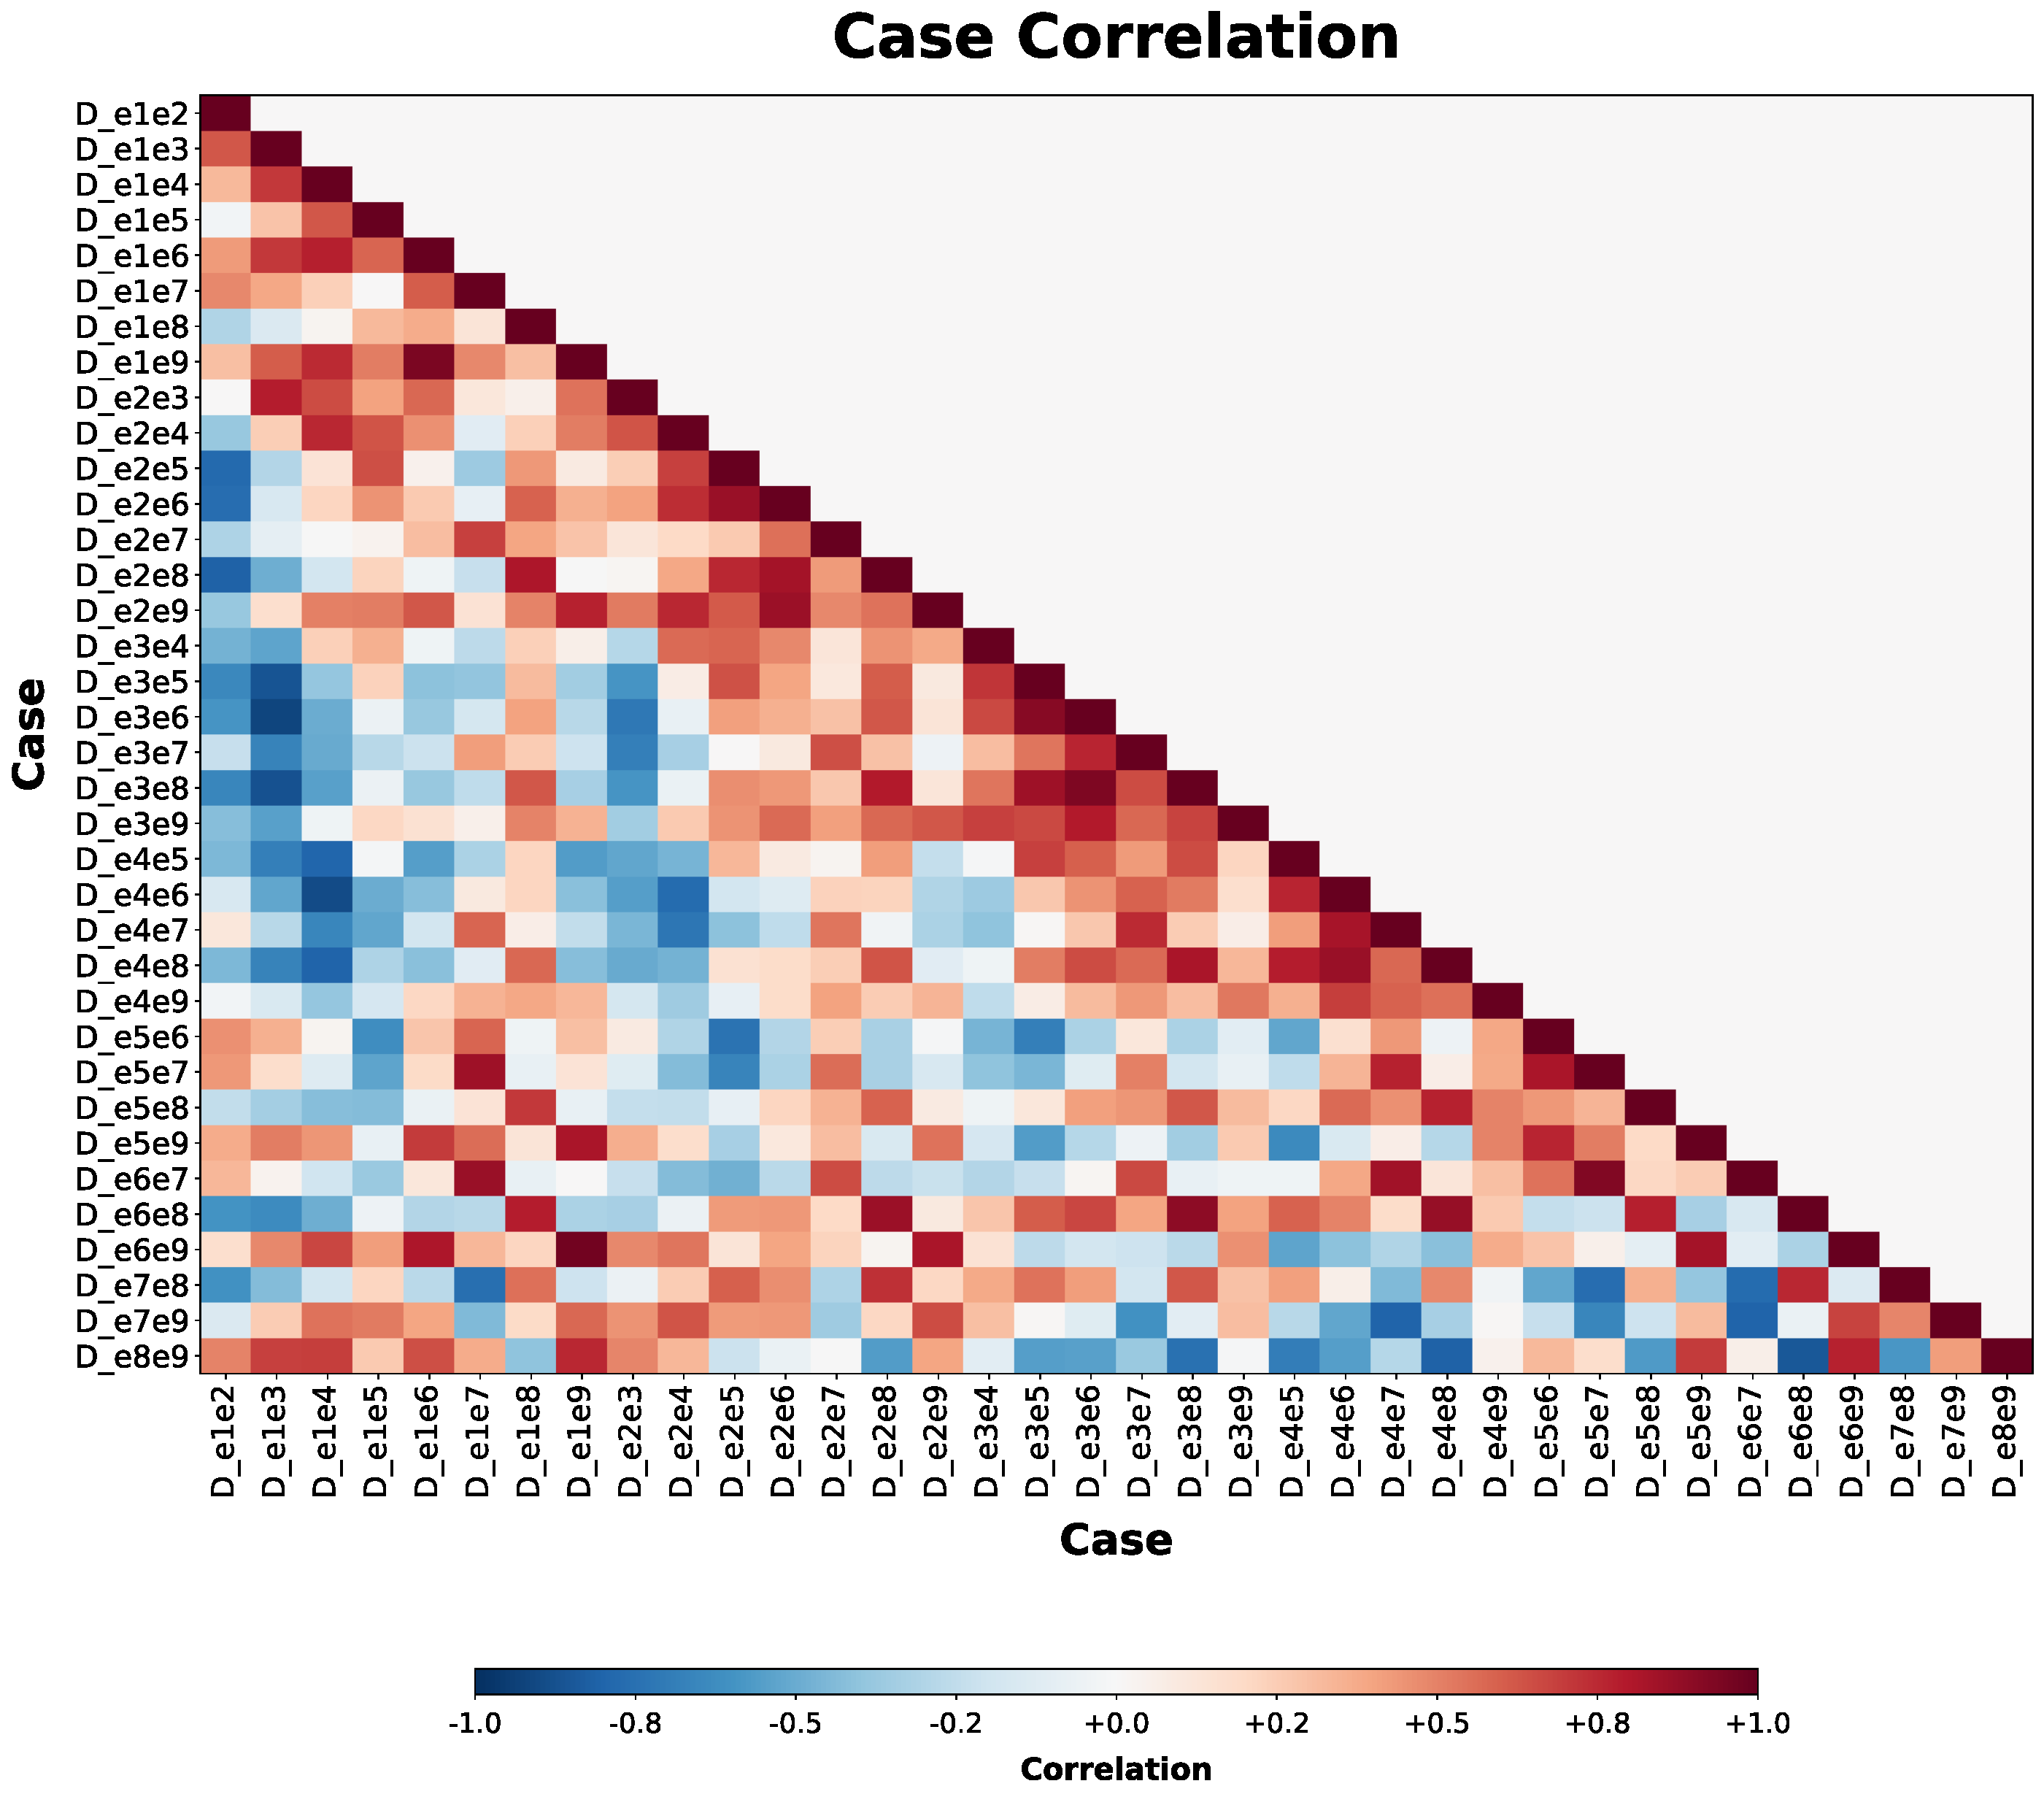
\includegraphics[width=\textwidth]{../../02_Images/dip_correlation_heatmap.pdf}
\caption{Correlation matrix for dipolar stimulation patterns.
Columns show lower correlation ($r \approx 0.31$), indicating more diverse probe patterns.}
\label{fig:dip-correlation}
\end{figure}

These results demonstrate that dipolar stimulation is the superior choice for the
following reasons:
\begin{enumerate}
  \item \textbf{Full spatial coverage}: It spans the complete 21-dimensional probe
        measurement space (rank 21 vs 9 for monopolar), enabling representation of
        arbitrary scalp potential patterns.
  
  \item \textbf{Superior spatial discrimination}: Probe responses show 15× higher
        variability across different source configurations (CV = 645\% vs 44\%),
        meaning the system can distinguish between different dipole activations much
        more effectively.
  
  \item \textbf{Directional encoding}: Dipolar fields encode spatial directionality
        through field gradients, providing richer information about source orientation.
  
  \item \textbf{Flexibility for optimization}: Starting with 36 dipoles to span a
        rank-21 space provides redundancy that can be leveraged during subset selection.
        This allows trading off some dipoles to improve the condition number while
        maintaining substantially higher rank than monopolar---a flexibility essential
        for balancing numerical stability with spatial coverage.
\end{enumerate}

In contrast, the monopolar protocol cannot provide full rank coverage of the measurement
space, fundamentally limiting its spatial discriminability.
